\subsection{Pattern architetturali} \label{subsec:architectural_patterns}
Il sistema è progettato seguendo il pattern architetturale Model-View-Controller (MVC), che separa le responsabilità tra la
logica del sistema (movimenti sul tabellone e vari minigiochi), l'interfaccia utente e la gestione degli eventi.
La scelta di MVC è motivata da quanto descritto nei requisiti di implementazione, in quanto consente di separare
le preoccupazioni tra la logica di gioco, l'interfaccia utente e la gestione degli eventi, facilitando così lo sviluppo,
la manutenzione e l'estensibilità del sistema; così facendo si allinea con i principi di un buon design software, che enfatizzano
la chiara descrizione e l'organizzazione delle responsabilità per evitare che l'implementazione sia percepita come
"accaduta senza ragioni e comprensione delle implicazioni".
Questo approccio consente una maggiore modularità e facilita la manutenzione e l'estensibilità del sistema. In particolare, la
separazione in Model, View e Controller rappresenta un esempio di "design architetturale" in quanto definisce gli aspetti strategici 
del design, la "bigger picture", e stabilisce i confini principali e i contratti tra le sottosistemi.
Non essendo un sistema distributo, non vengono utilizzati pattern architetturali specifici per la distribuzione e infatti sia
Model che View e Controller sono realizzati all'interno dello stesso processo.
Il Model rappresenta tutte le entità in gioco (tabellone, giocatori, dadi, mosse, struttura dei minigiochi), il Controller gestisce
gli eventi generati dall'utente e, modificando il Model, fornisce le informazioni necessarie alla View per aggiornare l'interfaccia
utente. Per come è strutturato il sistema, la View è sia punto di visualizzazione che punto di interazione con l'utente, in quanto
l'utente interagisce con il sistema attraverso l'interfaccia grafica. Il successivo design dettagliato di ciascun componente
(Model, View, Controller) potrà poi avvalersi di design patterns specifici, idiomi di programmazione e refactoring per organizzare
formalmente il codice, concentrandosi sugli aspetti tattici e sul "smaller picture" dell'implementazione.
Il diagramma della struttura del sistema viene mostrata nella Figura \ref{fig:architectural-patterns}.
\begin{figure}[H]
    \centering
    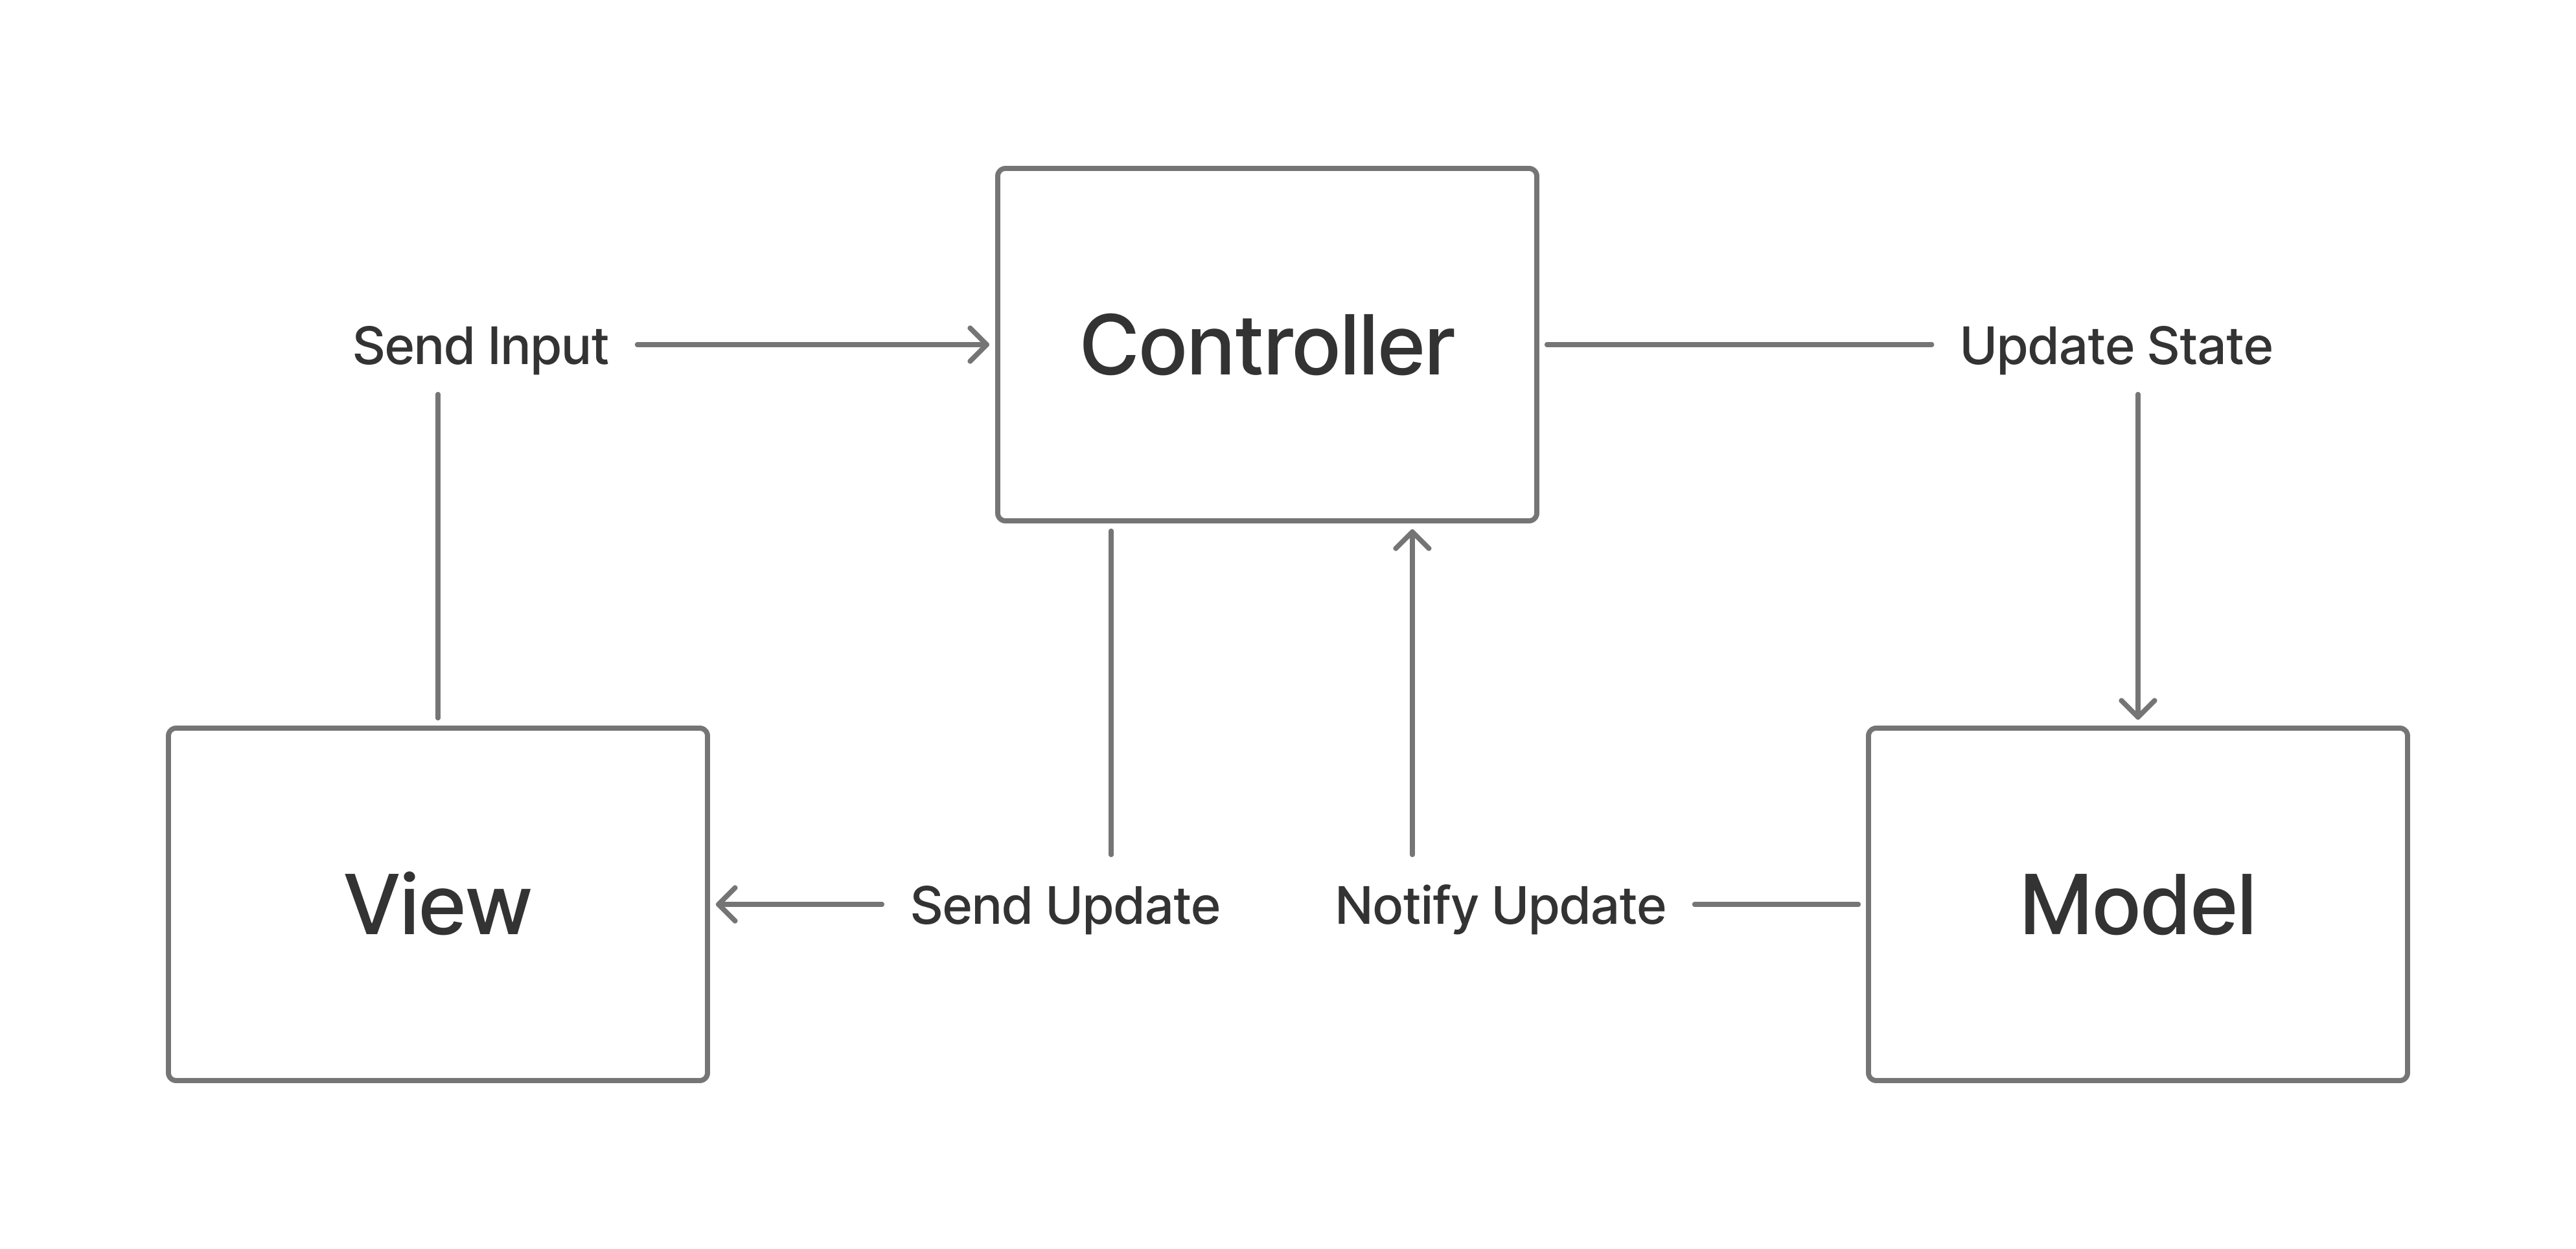
\includegraphics[width=0.8\textwidth]{images/MVC.png}
    \caption{Struttura MVC del sistema}
    \label{fig:architectural-patterns}
\end{figure}
Come si può vedere dalla figura, il Model effettua una notifica al Controller quando ha terminato l'aggiornamento ricevuto da
quest'ultimo, in questo modo la View non ha dipendenza diretta dal Model, ma solo dal Controller e si riesce a manatenere tutto
il sistema disaccoppiato.
